\section{Introduction}
Matched-field processing (MFP) is a common technique for source localization in a underwater
wave-guide\cite{bucker1976use,baggeroer1988matched,baggeroer1993overview},
which matches measured acoustic pressure field data on an array of sensors with a replica field computed by a numerical propagation model for an assumed source range and depth. The processor output is maximum at the true source range and depth. However, MFP requires a pretty good knowledge of environment, thus significant errors in the environment model can be introduced into the
depth and range localization predictions\cite{tolstoy1989sensitivity,del1988effects}.

Unlike MFP, machine learning methods do not require a good \emph{a prior} information and can implement a required calculation through learning from examples, Furthermore, a well designed structure can learn a generic model that works in different kinds of scenarios. This is meaningful for us to improve the robustness of matched-field source localization by introducing machine learning methods into underwater acoustics.
Machine learning  has obtained success in many areas, such as speech recognition, natural language processing and image processing. There are also applications of machine learning in underwater acoustics.
For example, previous works have used artificial neural networks to classify whale sounds\cite{thode2012automated}, locate targets\cite{steinberg1991neural} and discriminate depth\cite{ozard1991artificial}.
A notable recent example using machine learning methods in underwater acoustic is the Niu's application of nonlinear classification to source localization\cite{niu2017source}. As far as we can tell, there is no discussion on how to use a machine learning method to help solve the mismatch problem in underwater source localization.

In this paper, the source localization problem is viewed within a machine learning framework, and a method that can tolerate the mismatch problem is proposed.
As the sound-speed profile (SSP) in the water layer is the most important parameter needed to be known accurately\cite{feuillade1989environmental}, we primary focus on the SSP
mismatch problem.
In our simulations, two different degrees of error (a large one and a slight one) in the knowledge of the sound-speed profile are chose to train and test the model.
%The large one has significant change in shape, while the slight one just has small shift (within 0.5m/s at the same depth) in sound speed.
Effects of such errors on positioning performance for various methods, including Bartlett matched-field processing, matched-covariance estimation (MCE) and SCFNN, are compared.
Treat different SSPs as different application scenarios, and then a generic model is learned by data-model mixed training, the trained model is tested on
varying SSPs.
In Niu's work\cite{niu2017source}, he used a dense neural network to train his model, and his model performs well on the data of Noise09 experiment, which verified that FNN can achieve a good prediction performance when source localization is solved as a classification problem. However, as the author said, the FNN classifier will be over-fitting when the SNR of training data is low, i.e. the model accuracy on training set is much lower than test set. In order to overcome this problem,
a SCFNN is used in this paper. Besides, our models are trained and tested on SWellEx-96 experimental or simulated data.

\section{Sparse Neural Networks Based Source Localization}
In this section, we discuss how to establish a SCFNN for
source localization prediction and how to train it with mixed data-model.

\subsection{Neural networks and function approximation}
As we known, neural networks models can be viewed as a mathematical function $f$. Taking feed-forward neural network (FNN) as an example, it defines a mapping ${{y}}=f(x;\theta )$ between the input $x$ and the output $y$ by parameter $\theta$, where the parameters are needed to be learned by a rule. FNN is typically represented by composing together many different functions. There might have two function $f^{1}$, $f^{2}$ connected in a chain\cite{goodfellow2016deep}, to form
$f(x) = f^{2}(f^{1}(x))$.

\subsection{Source localization prediction model}
In his paper\cite{niu2017source}, Niu assumed that there is a deterministic relationship between source range and sample-covariance matrix (SCM) and approximated this relationship by the FNN. Same as Niu did, we also use FNN to approximat the relationship between
source range and SCM in this paper.

FNN extends linear models to represent nonlinear transformed format $\phi(x)$ of the input $x$. The transform function $\phi$ defines a hidden layer $h=\phi(x)$ and can be regarded as providing a set of features describing $x$, or as providing a new representation for $x$. The crucial problem here is how to choose the transform function $\phi$. As the people engaged in machine learning usually do, we use a linear combination with nonlinear function to fit the basis functions,
\begin{equation}
h = g(W^{(1)}x + b^{(1)})
\end{equation}
Neurons between the hidden layer and the output layer are simply mapped by a linear function,
\begin{equation}
z = {W^{(2)T}}h + {b^{(2)}}
\end{equation}
Then the output of the model is normalized by $ softmax $ function, which is a common choice for multi-class classification task\cite{bishop2006pattern},
\begin{equation}
p({y_k}|x) = softmax {(z)_k} = {{\exp ({z_k})} \over {\sum\nolimits_j {\exp ({z_j})} }}
\end{equation}
where $x$ is the input data, $p({y_k}|x)$ is the probability that measured signal $x$ transmitted from position $k$. $W$ and $b$ in Eq.(1) and Eq.(2) are the parameters needed to be learned.

Obviously, a criterion is needed. In most cases, the parametric model defines a distribution $p(y|x;\theta)$ and we can simply use the principle of maximum likelihood to determine the parameters in this model,
\begin{equation}
J(\theta ) =  - {E_{x,y \sim {p_{data}}}}\log {p_{model}}(y|x)
\end{equation}
As the maximum likelihood criterion is consistent, the model is capable of representing the training data distribution.

\subsection{Training the model with sparsity constraint and mixed data-model}
\emph{\textbf{A. Sparsity constraint on neural networks}}

A SCFNN can be easily got by adding sparsity constraint on networks and there are two main kinds of sparsity methods, including weight-level regularization and neuron-level regularization\cite{goodfellow2016deep},
\begin{equation}
\tilde J(\theta ;X,y) = J(\theta ;X,y) + \alpha \Omega (\theta )+ \beta \Omega (h)
\end{equation}
where the $\Omega (\theta )$ is weight decay term and $\Omega (h)$ is penalty on the activations of the units, $\alpha$,$\beta$ are hyper parameters that control the relative contribution of
the two penalty term. Weight decay term penalizes the size of the model parameters, while, the activation penalty term encourages their activations to be sparse and makes the neural network to be sparsely coded.
A sparsely-coded neural network encodes each input data as a sparse code firstly, and then accomplish the specific task with further processing.

In practical applications, we not only want the network to be sparse, but also want the model parameters to be sparse, the latter makes the model more interpretable. In this paper, we use $L_{1}$-norm to promote sparse neurons activations, and constrain the $L_{2}$-norm of each column of the weight matrix to prevent any one hidden unit from having very large weights. The objective function modified as below,
\begin{equation}
\begin{split}
&\tilde J(\theta ){\kern 1pt} {\kern 1pt} {\kern 1pt} {\rm{ = }}{\kern 1pt} {\kern 1pt} {\kern 1pt}  - {E_{x,y \sim {p_{data}}}}\log {p_{model}}(y|x){\rm{ + }}{\kern 1pt} {\kern 1pt} \lambda {\left\| h \right\|_1}\\
& s.t.{\kern 1pt} {\kern 1pt} {\kern 1pt} {\kern 1pt} {\kern 1pt} {\kern 1pt} {\kern 1pt} {\kern 1pt} {\kern 1pt} {\kern 1pt} {\left\| {{W^{(1)}_i}} \right\|_2} \le C{\kern 1pt} {\kern 1pt} {\kern 1pt} {\kern 1pt} {\kern 1pt} {\kern 1pt} {\kern 1pt} {\kern 1pt} {\kern 1pt} \forall {\kern 1pt} i = 1, \cdots ,M\\
\end{split}
\end{equation}
where, $M$ is the number of the neurons in hidden layer, $C$ is the constraint coefficient,which does't matter much here, and we choose $C=1$ in our simulations.

\leftline{\emph{\textbf{B. Data-model mixed training}}}

Another strategy used in this paper is training the model with mixed data-model, in order to increase the model robustness.
As neural networks are strong enough to learn regular pattern over a set of changing scenarios,
when training the model, we can use the examples gathered form different mismatch scenarios to make the model be robust to mismatch problem. In our case, the mixed model data, i.e. the receive acoustic pressure data computed by various environment models, are combined as the training set.

Neural network models are easily to be over-learning, because of their powerful fitting ability and the noisy, discrepant data samples. Thus, sparsely-coded neural network is much more necessarily to be applied in data-model mixed training cases.

\section{Simulation and experimental results}
In this section, the SCFNN implemented above is used to learn the source range directly from the data of the SWellEx-96 experiment, and the performance of the classifier is compared with some other matched-field processing methods in terms of simulation data or experimental data, respectively. In addition, the influence of SSP mismatch on the performance of SCFNN classifier is investigated by simulations. In our application,the robustness of the classifier is improved by training the model using data sampled under different SSP.

Simulation environment is the widely studied SWell96-Ex test, conducted in a shallow water waveguide environment with 216 m in depth.
During the experiment, two moving sound sources are deployed in field, including a deep source (J-15) and a shallow source (J-13). In all of the following simulations, the shallow sound source is used, which was towed about 9 m in depth and emitted with 9 frequencies between 109 Hz and 385 Hz. The number of vertical array elements $L$ is 21, and other specific deployment parameters is shown in Fig. 2.

\subsection{Parameter settings}
In simulation part, acoustic data used to train and test the neural network is simulated using kraken\cite{porter1992kraken} with environment models. The normalized SCMs of measured pressure at each frequency is used as model input data. In input layer, number of neurons $D$ is $L^{2} \times N_{fre}$(number of frequency used) and the number of neurons in the output layer (number of classes) is $K = 300$. Simply, the number of neurons in hidden layer is set to be equal to the input layer, i.e. $M = D$. During the input data preprocessing, fast fourier transform duration is 1-seconds and snapshot $N_{s}$ for constructing SCMs is 10.
%The objective function now becomes
%\begin{equation}
%{\kern 1pt} {\kern 1pt} {\kern 1pt} {\kern 1pt} {\kern 1pt} {\kern 1pt} \tilde J(\theta ){\kern 1pt} {\kern 1pt} {\kern 1pt} {\rm{ = }}{\kern 1pt} {\kern 1pt} {\kern 1pt} {\rm{ - }}{{\rm{1}} \over N}\sum\limits_{n = 1}^N {\sum\limits_{k = 1}^K {{t_{nk}}\ln {y_{nk}}{\kern 1pt} {\kern 1pt} {\kern 1pt} {\rm{ + }}{\kern 1pt} {\kern 1pt} \lambda {{\left\| h \right\|}_1}} }
%\end{equation}
%where $t_{nk}$ and $y_{nk}$ are the practical and the predictive probabilities of the sample data $x$ belonging to the $k$-$th$ class separately and we choose $C=1$ here.
For the sake of learning speed and sparsity of hidden neurons, $ReLU$ activation\cite{goodfellow2016deep} is applied in hidden layer.
The training set contains 3000 samples sampled uniformly with 1.82\--8.65 km in range, the test set is another 300 data sampled with the same range. All of the noise in the simulations is set to be complex gaussian white noise.
\begin{figure}
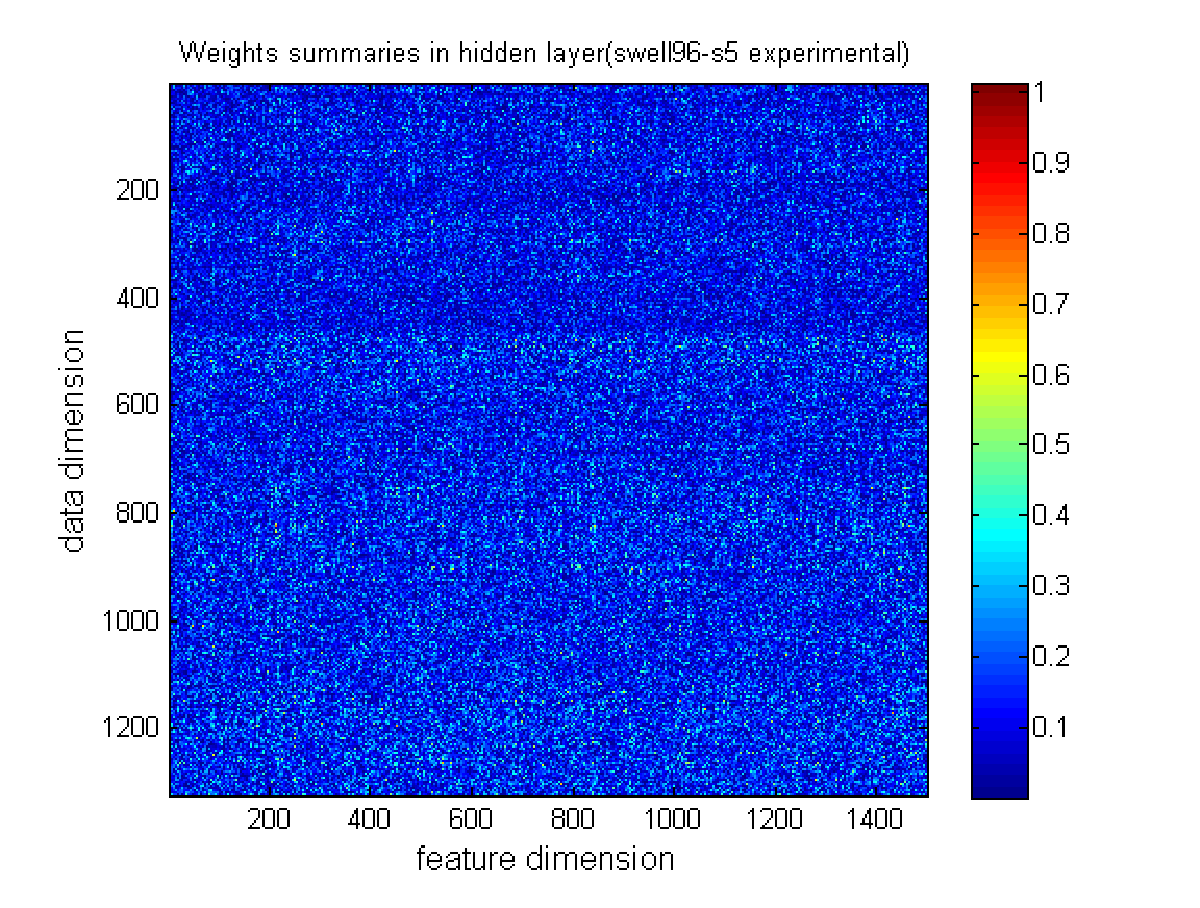
\includegraphics[width=4cm,height=3cm]{figure/Weights_summaries_in_hidden_laye_swell_exp}
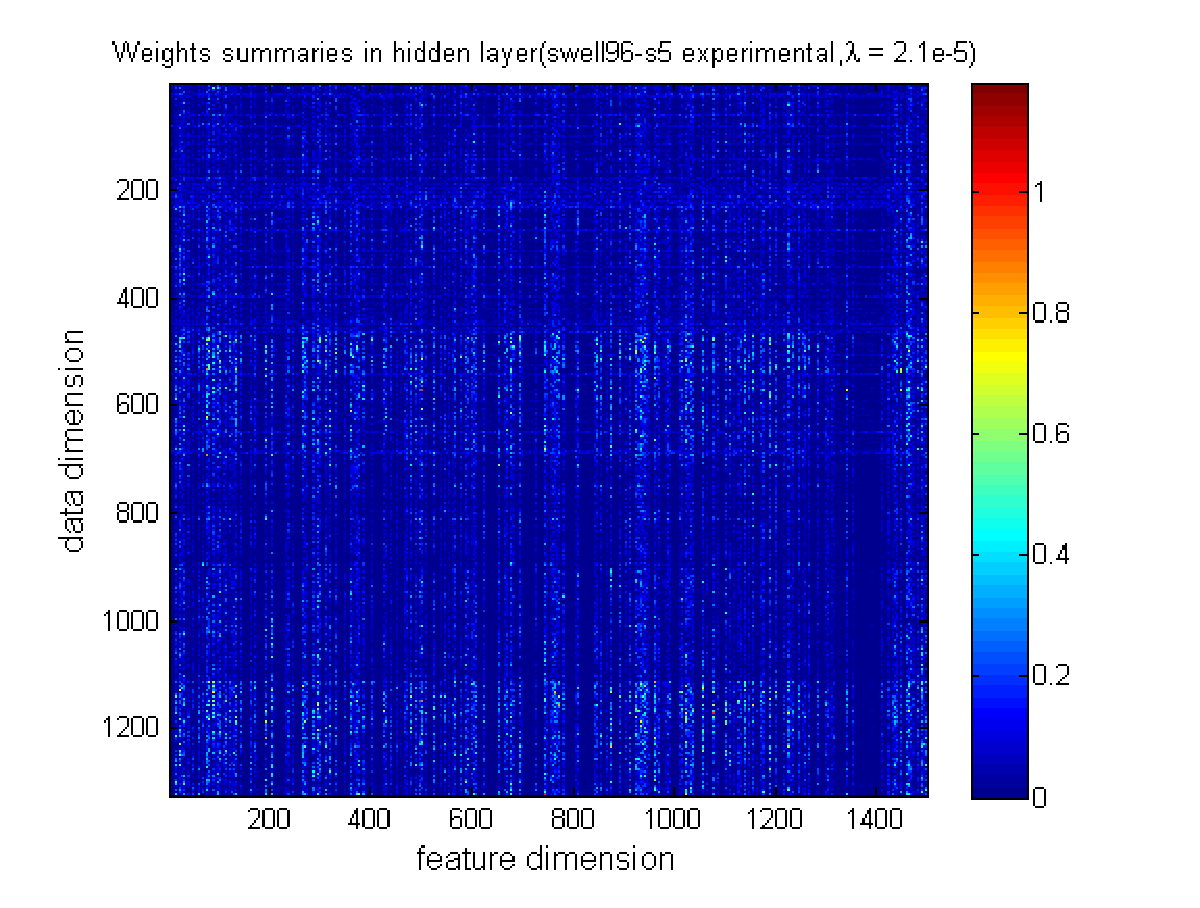
\includegraphics[width=4cm,height=3cm]{figure/Weights_summaries_in_hidden_layer_swell_exp_lambda_2_dot_1e_neg_5}
%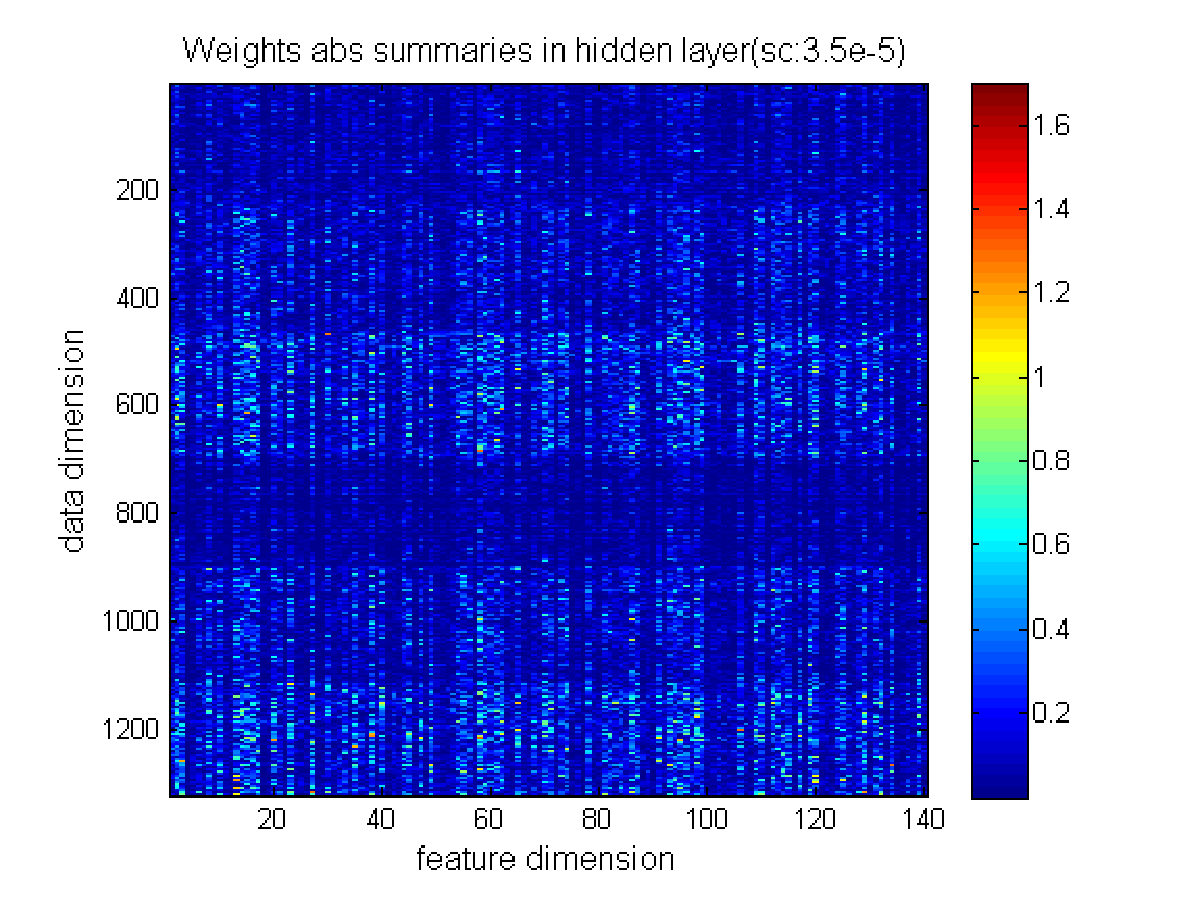
\includegraphics[width=4cm,height=3cm]{figure/Weights_abs_summaries_in_hidden_layer_sc3dot5e_nag_5_swell_140}
%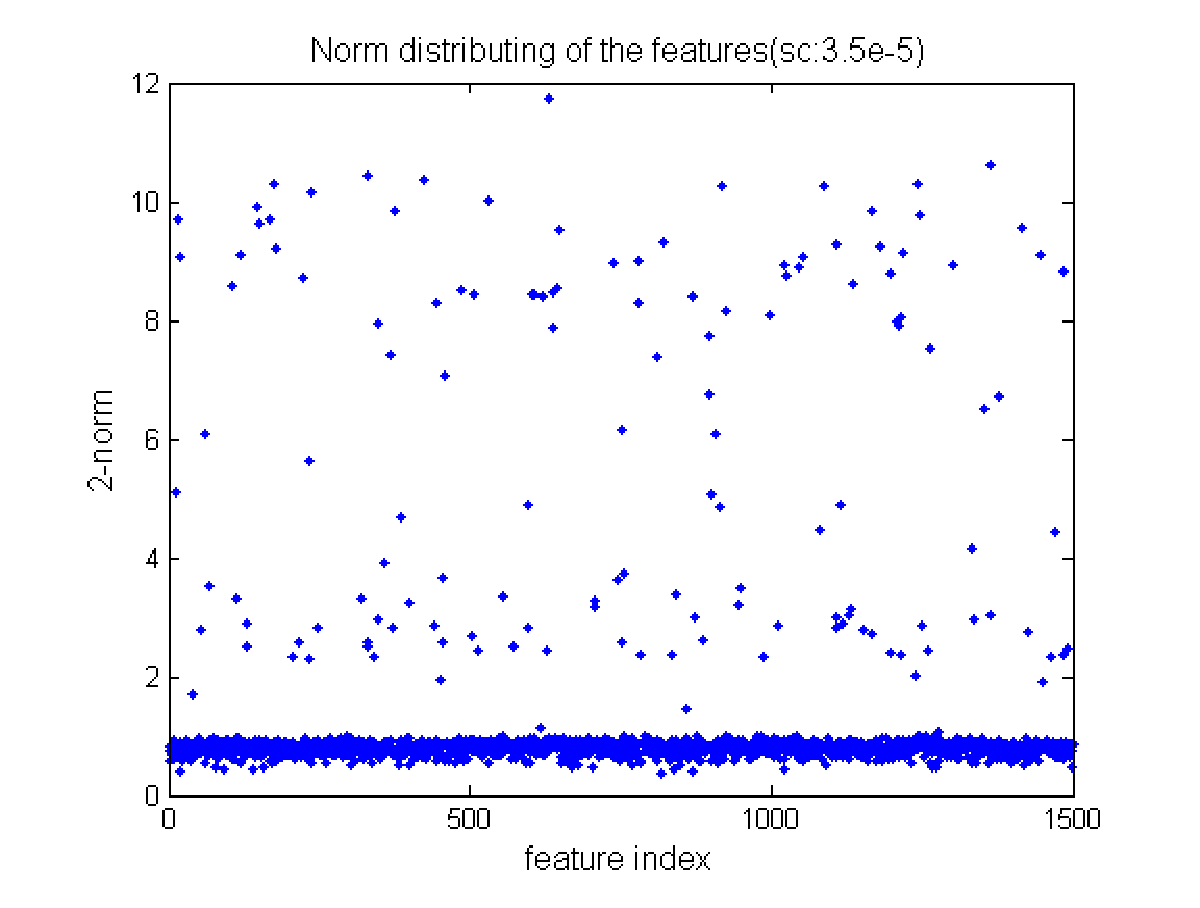
\includegraphics[width=4cm,height=3cm]{figure/Norm_distributing_of_the_features_sc3dot5e_nag_5_swell}
\caption{Weights summary in hidden layer (left: no constraint, right: with constraint). Sparse constraint
training makes the weight coefficients show group structure, either all zero, or basic is not zero.}
\end{figure}
Experimental data is got from SWell96-Ex Event S5 vertical line array (VLA). The array recorded a total of 75 minutes data. In order to facilitate processing, 0\--50 min data is took as a training set.
Consistent with the simulation part, the experimental trajectory was divided into 300 grids, 25 m each in range. The snapshot is also set as 1-second and finally 3000 SCMs would be got. Each SCM is averaged at every two snapshots, 2700 of the samples are took as the training set and the remainder as test set.
\begin{figure}
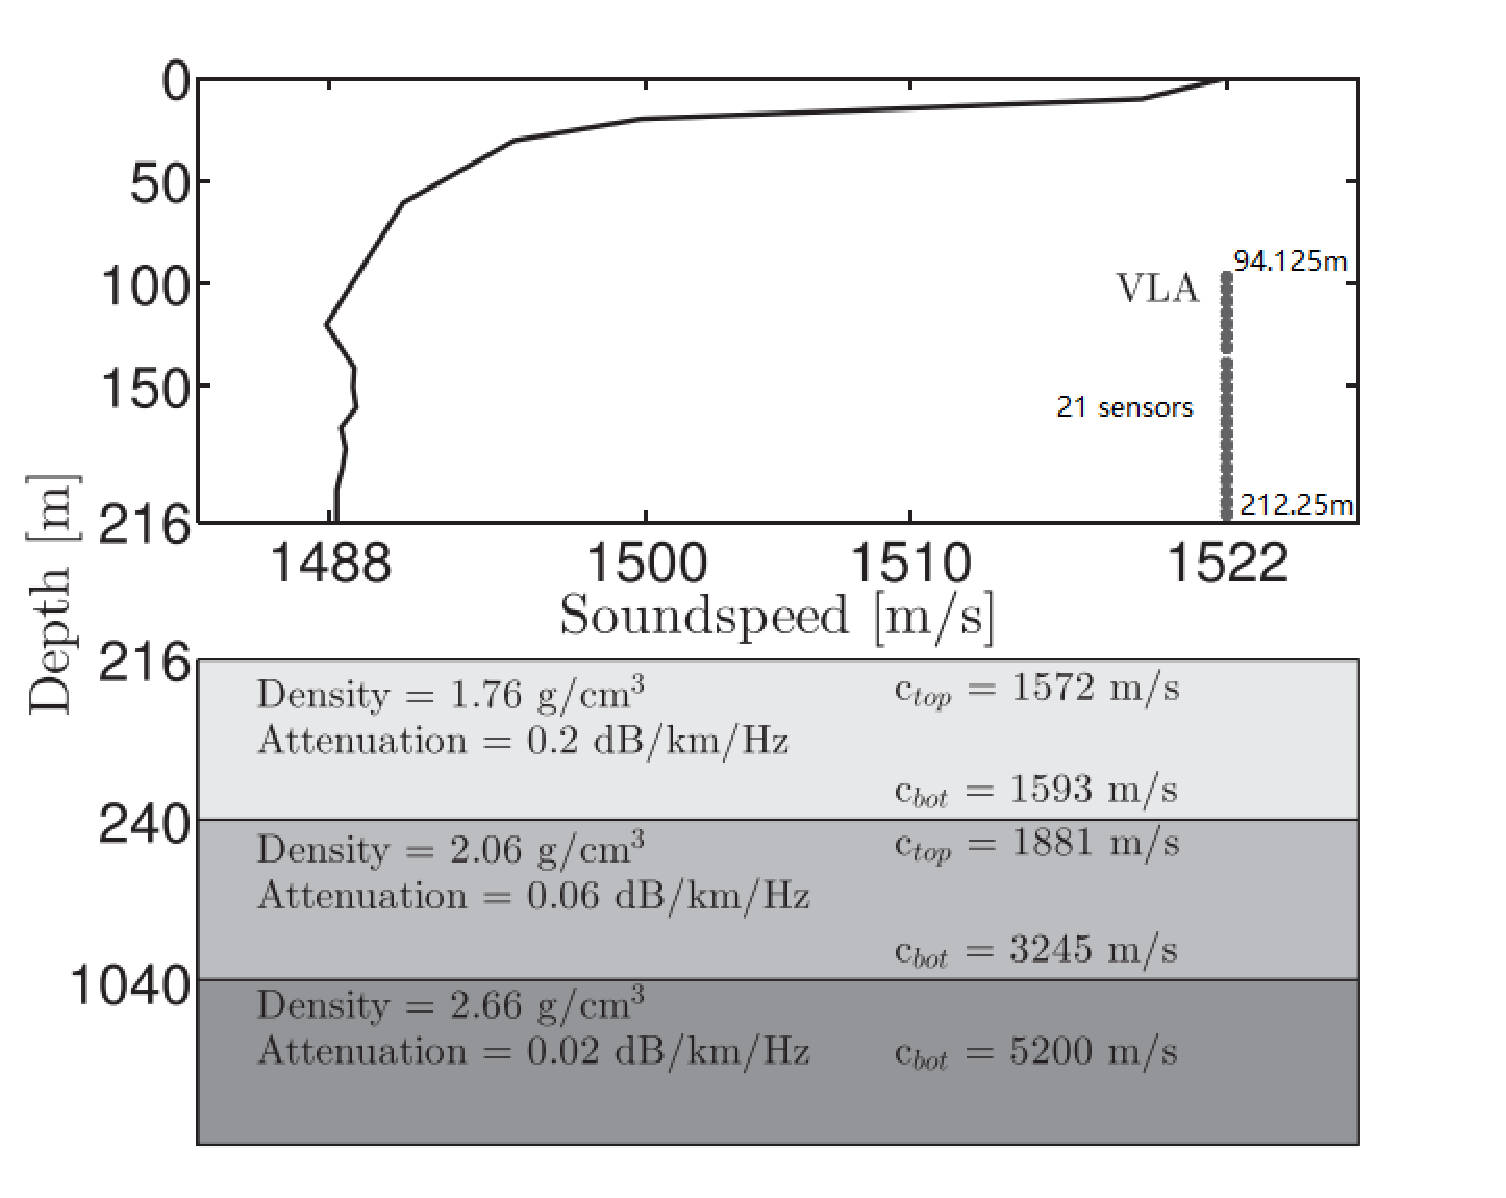
\includegraphics[width=8cm]{figure/environment}
\caption{Environment. An impressively detailed \\environment model for SWellEx-96 experiment.}
\end{figure}
\subsection{The effect of sparsity constraint training}
As shown in Fig. 3, the SCFNN efficiently prevents the model from over-learning, i.e. no over-fitting occurs.
Besides, we can also find that the regularization degree on model affects the model accuracy and the average activation density of FNN's hidden layer. As the coefficient grows, the model accuracy on training set and test set also drops,
%drops fastly on the training set, while slower on the test set.
and when the coefficient is too big, the model accuracy on training set becomes much lower than test set, which indicates under-fitting.
The optimal coefficient $\lambda$ in this paper is manually chosen by testing.
%The model error is defined as the dissimilarity between true probability distribution and estimated probability distribution, thus the Kullback-Leibler(KL) divergence.
%In Fig.2, we use the cross entropy equivalently.
On the other hand, as the coefficient grows, the order of magnitude on average activation drops from $10^{3}$ to $10$, and keeps stable. This is good for us to train a SCFNN.

Compared to the case of training without sparse constraints, SCFNN makes the weight coefficient in the hidden layer show group structure, i.e. the element of weight vector is either all zero, or basic is not zero.
It can be seen that the relative size of learned weights in hidden layer is related to the frequency, as we can see bright and dark strips can be seen distributed along the data dimension (input data dimension arrangement is relative to frequency) in Fig. 1.
%and even at the same frequency, the weight corresponding to real and imaginary parts is also different, as we can see bright and dark strips can be seen distributed along the data dimension (input data dimension arrangement is relative to frequency) in Fig. 1.
%(when we plot the weights summaries, the data dimension is arranged according to the frequency relationship from 109 Hz to 385 Hz.)
In our model, we choose $\lambda=2.1 \times 10^{-5} $, and the number of feature vectors in hidden layer reduces from 1500 to 740, as shown in Fig. 1. At the same time, the average activation neuron number in hidden layer is just 16 and the activation rate is only 1.1{\%}.
\begin{figure}
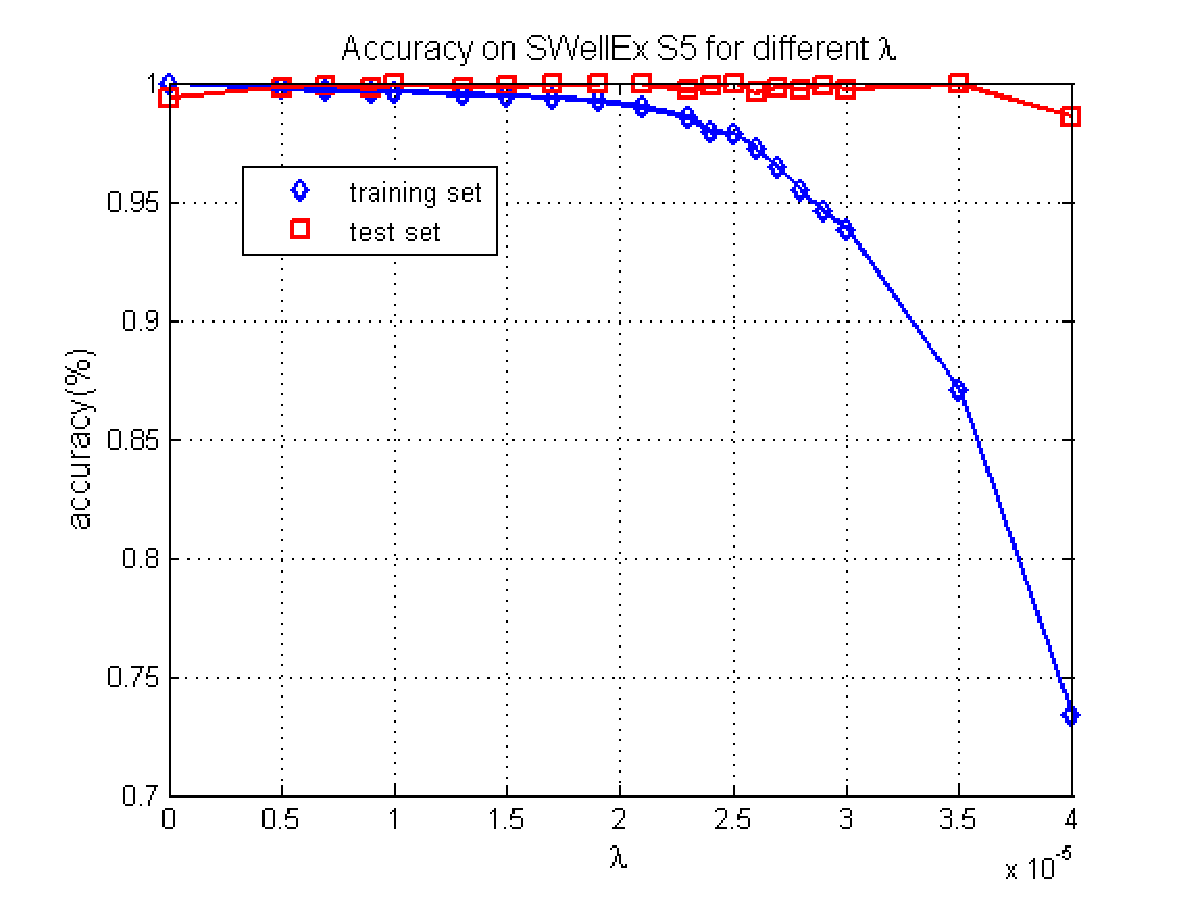
\includegraphics[width=4cm,height=3cm]{figure/Accuracy_on_SWellEx_S5_for_different_lambda}
%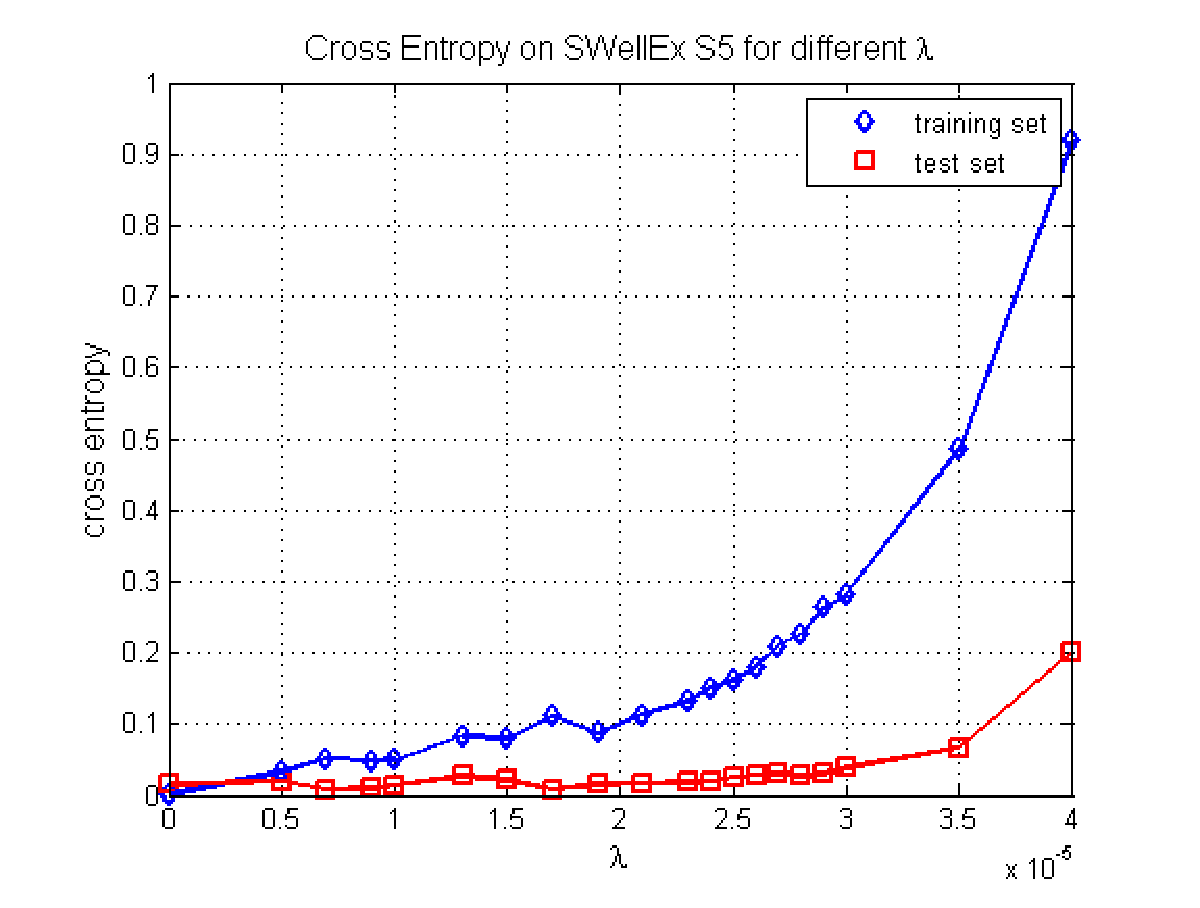
\includegraphics[width=4cm,height=3cm]{figure/Cross_Entropy_on_SWellEx_S5_for_different_lambda}
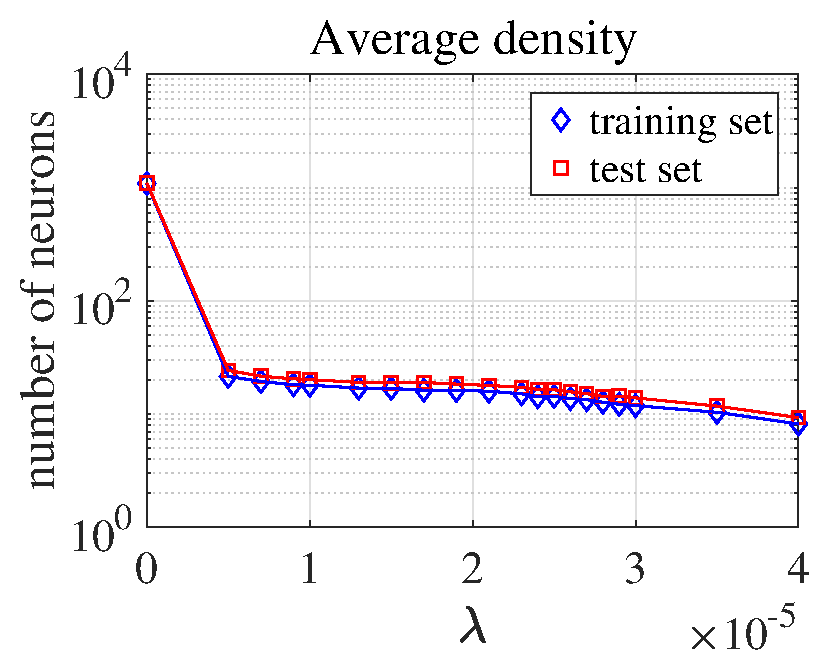
\includegraphics[width=4cm,height=3cm]{figure/Hidden_Average_Density_on_SWellEx_S5_for_different_lambda}
\caption{Model accuracy and Average-activation-density for different $\lambda $. Regularization on neuron-level
significantly reduces the average activation density and achieves good model accuracy. The model is trained on SWell96Ex-S5 experimental data.}
\end{figure}
%\begin{figure}
%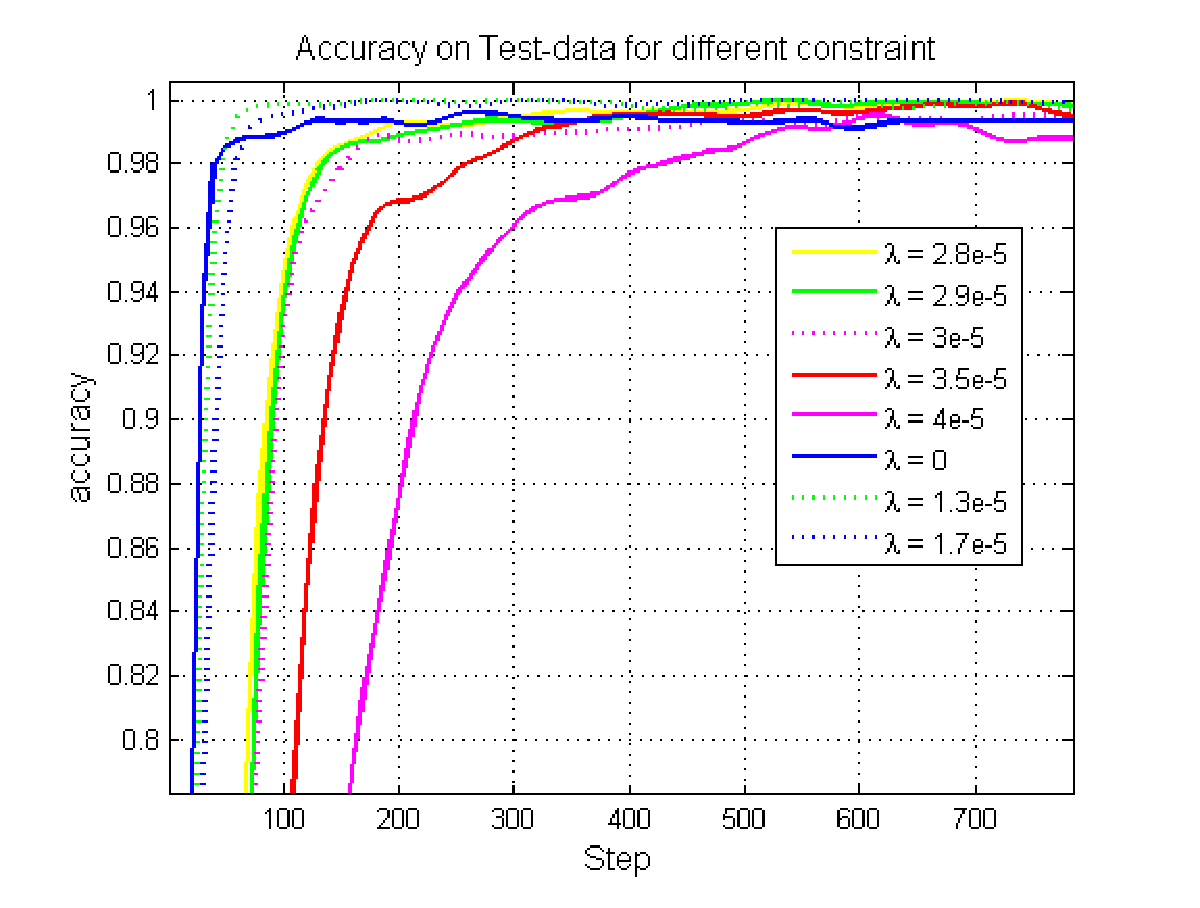
\includegraphics[width=4cm,height=3cm]{figure/Accuracy_on_Test_data_for_different_constraint_exp}
%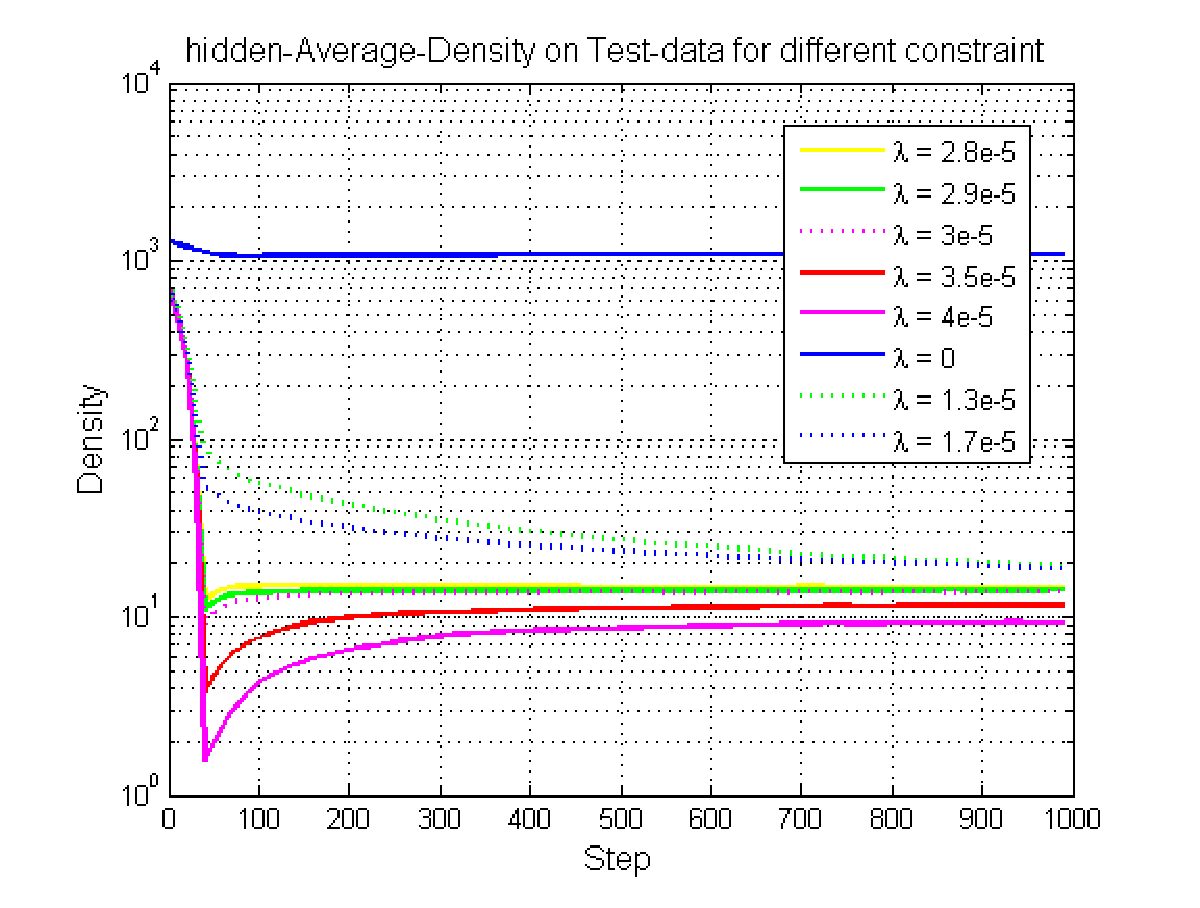
\includegraphics[width=4cm,height=3cm]{figure/hidden-Average-Density-on-Test-data-for-different-constraint_exp}
%\caption{Accuracy and Average-Density on test data for different-constraint.}
%\end{figure}

%\begin{figure}
%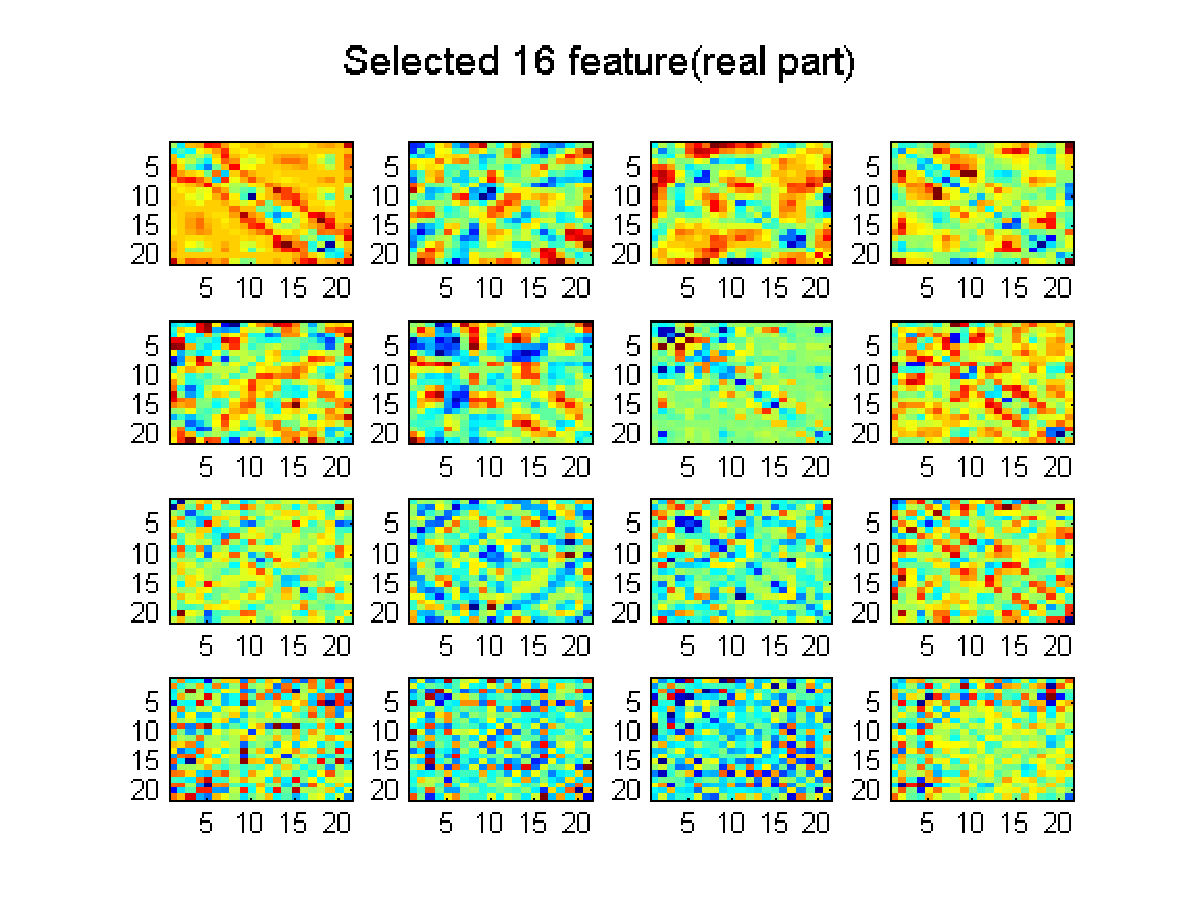
\includegraphics[width=4cm,height=3cm]{figure/selected_16_features_real_part}
%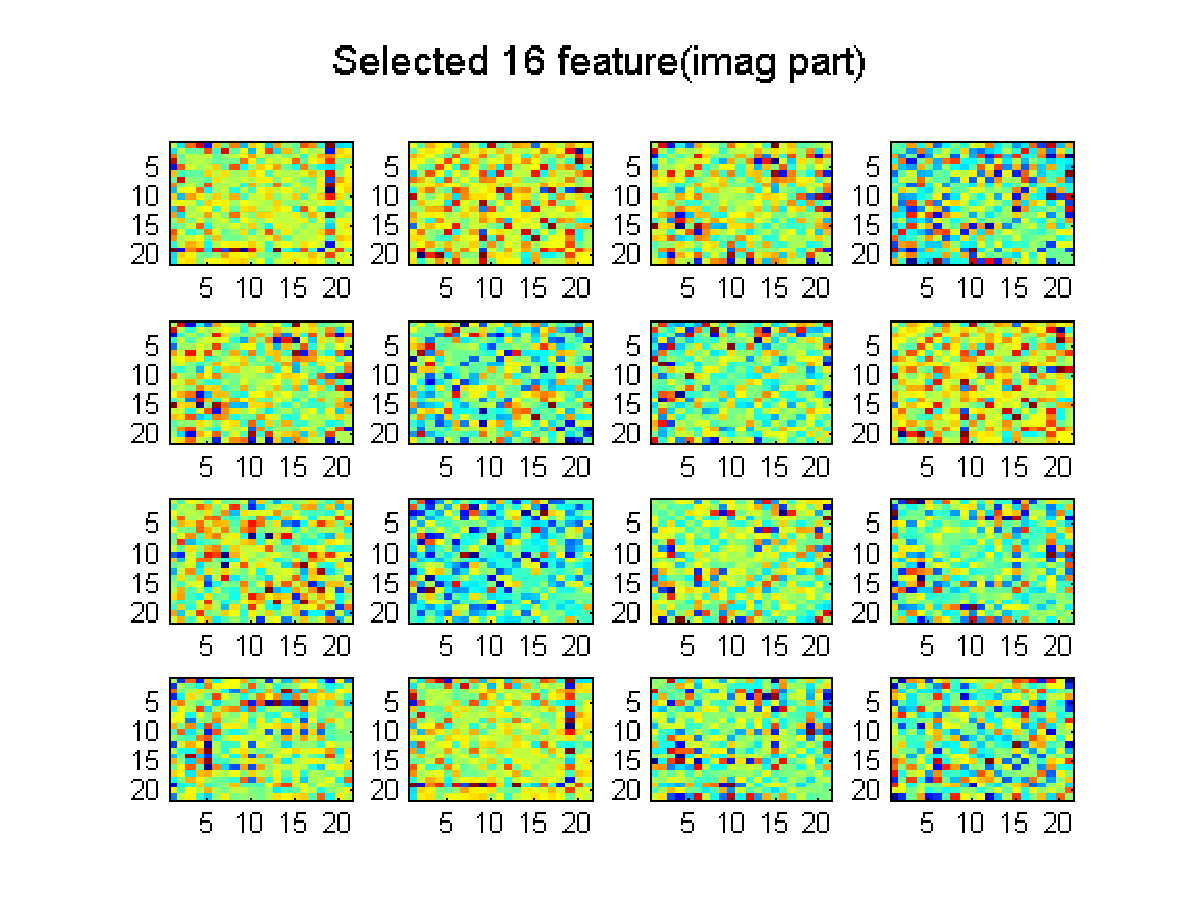
\includegraphics[width=4cm,height=3cm]{figure/selected_16_features_imag_part}
%\caption{Selected 16 features learned by neural network.}
%\end{figure}
\begin{figure}
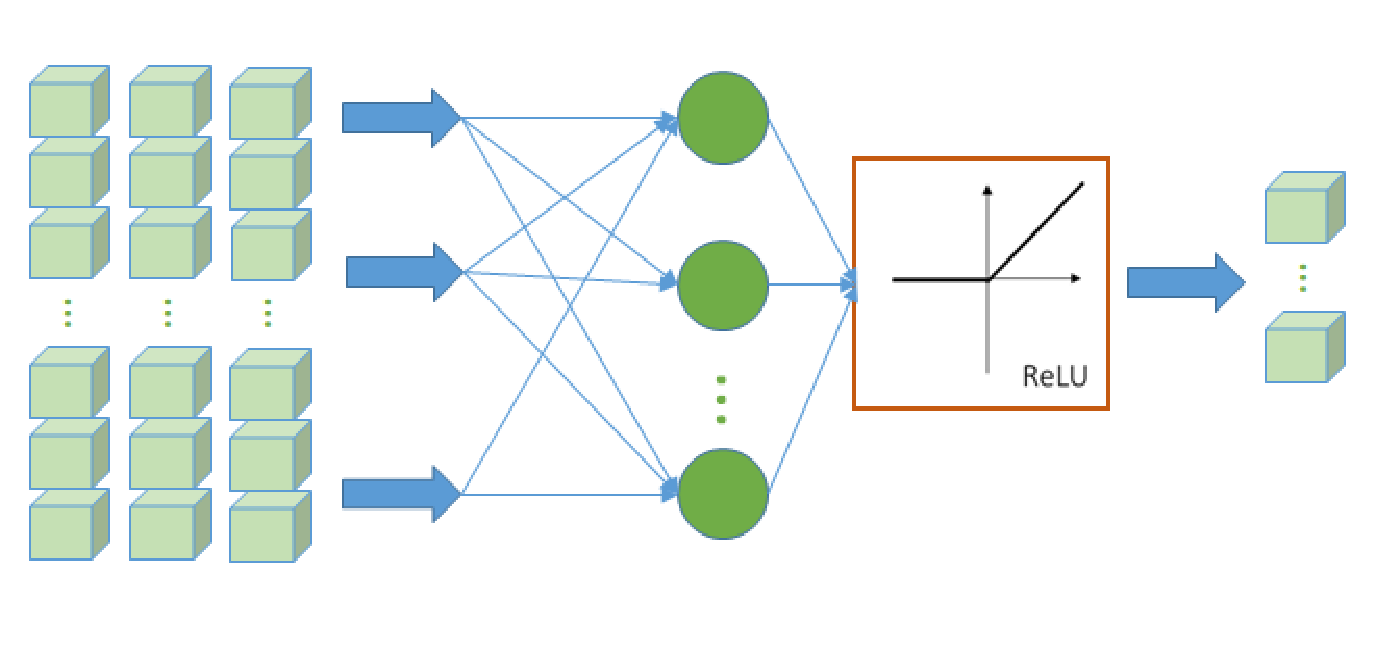
\includegraphics[width=8cm]{figure/sparse_represention_model}
\caption{The learned sparse representation model. The learned feature space spans data(scm) space likelihood that few basis functions $\phi$ explains a given data.}
\end{figure}
%Apart from being beneficial to feature selection, sparse constraint also reduces the activation rate of neurons in the hidden layer.
To sum up, by using regularization strategy on neural networks, a sparse and low rank model is builded, where the transferred representation is sparse and the rank of learned weight matrix is low. In our example, the input 1323-elements SCM data space can be spanned by the 740 feature vectors, and averagely, each data sample can be represented by only 16 feature.
This maybe useful for designing a decentralized source localization algorithm, where a sparse vector can be formed by filtering the data measured in sensor nodes through the pre-trained sparsely-coded neuron networks and source localization can be made in a fusion center.
%The learned sparse coding model is illustrated in Fig. 4.

%Decisions, such as target location can be made by further processing.
\subsection{Comparison with conventional matched-field processing method}
As a comparison, Bartlett processor is used here as a kind of MFP to positioning the source.
%as Niu did in his work.
There are two main kinds of replica-field used in the Bartlett processor, one is simulated by kraken (noted as bartlett 2), the other is the measurement data (noted as bartlett 1), same as the training data used in SCFNN.
% Please add the following required packages to your document preamble:
% \usepackage{booktabs}
\begin{table}[]
\caption{Localization accuracy of SCFNN and MFP on SWell96Ex-S5 experimental data}
\label{my-label}
\begin{tabular}{@{}lllll@{}}
\toprule
Methods       & SCFNN    & MCE    & Bartlett 1 & Bartlett 2 \\ \midrule
109Hz         & 89.3\% & 72.3\% & 37.7\%     & 3.7\%      \\
232Hz         & 97\%   & 91\%   & 17.7\%     & 4.3\%      \\
385Hz         & 99.7\% & 97.7\% & 14\%       & 0.67\%     \\
109,232,385Hz & 99\%   & 99.7\% & 40.7\%     & 7.7\%      \\ \bottomrule
\end{tabular}
\end{table}
% Please add the following required packages to your document preamble:
% \usepackage{booktabs}
\begin{table}[]
\caption{Absolute mean error of SCFNN and MFP on SWell96Ex-S5 experimental data(m)}
\label{my-label}
\begin{tabular}{@{}lllll@{}}
\toprule
Methods       & SCFNN  & MCE   & Bartlett 1 & Bartlett 2 \\ \midrule
109Hz         & 28.1 & 290.3 & 852.8      & 1219.5     \\
232Hz         & 7.4  & 2.5   & 832.3      & 832.3      \\
385Hz         & 0.08 & 0.58  & 1266.7     & 1756.3     \\
109,232,385Hz & 0.25 & 0.083 & 477.2      & 722.9      \\ \bottomrule
\end{tabular}
\end{table}
The accuracy and absolute mean error for different methods under different frequency are summed in table 1 and table 2. As we can see, whether in single frequency or in multi-frequency, the accuracy of SCFNN is always better than Bartlett, and not worse than direct data match (noted as MCE), this is more obvious when it comes to the comparison of absolute mean error.
It can be said that, the learned SCFNN works well on source localization and performs better than Bartlett processor.
\subsection{The influences of SSP mismatch on FNN classifier}
In the MFP method, the model accuracy is heavily affected by the mismatch problem\cite{tolstoy1989sensitivity,feuillade1989environmental,del1988effects}.
%Fig. 5 gives the FNN positioning results by simulations in different degrees change of SSPs. Herein, the snapshot is 10 and the SNR is 5dB.
\begin{figure}
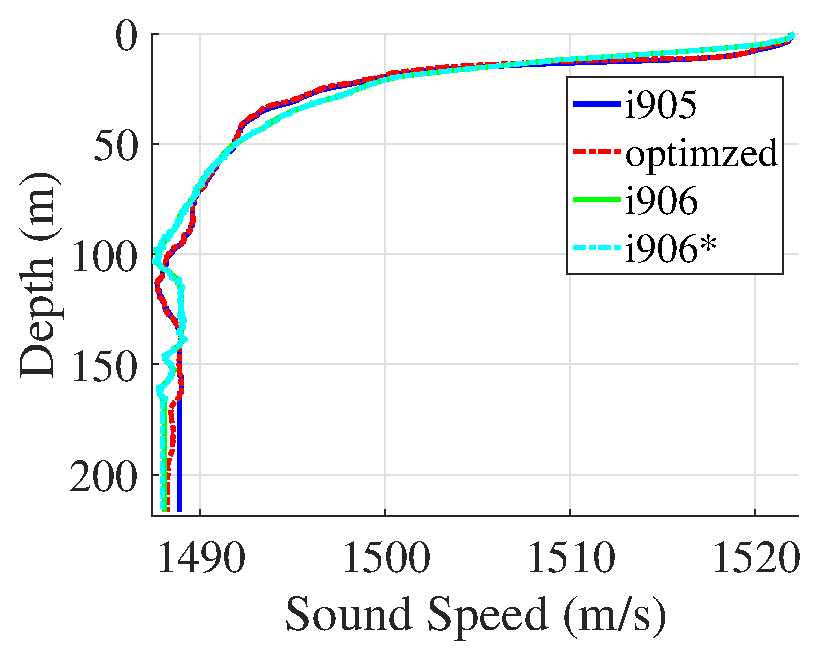
\includegraphics[width=6cm]{figure/ssp4}
\caption{Plots of sound speed profiles. The i906 has significant change in shape from the optimized, while the change in the i905 is slight. The i906{*} is little changed from i906, for the sake of testing.}
\end{figure}
%Comparing to optimized-ssp, the i905-ssp has only a very small change, within 0.5m/s at the same depth. The change in i906-ssp is much significant, which can be seen from the shape in Fig. 4.
\begin{figure}
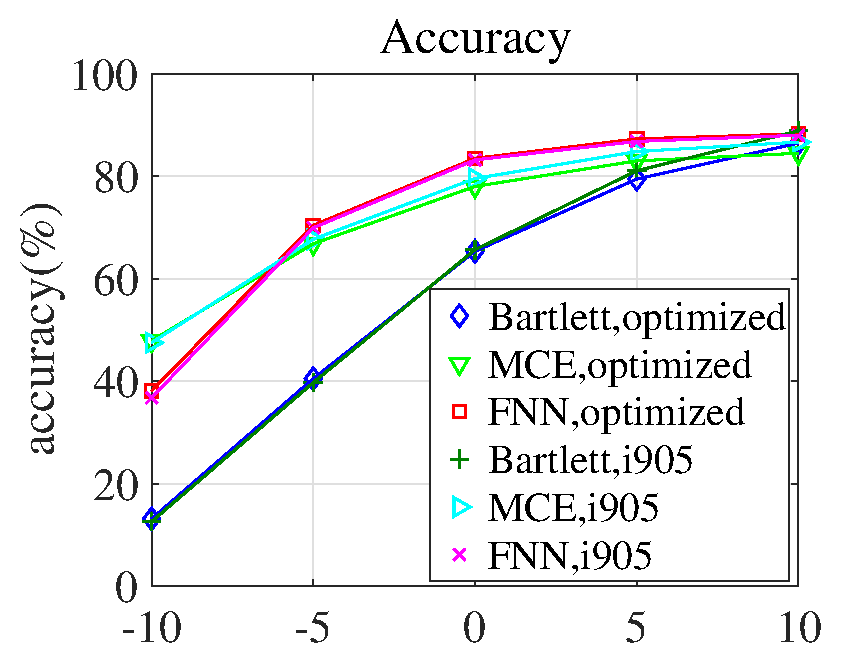
\includegraphics[width=4cm,height=3cm]{figure/Accuracy_to_SNR_FNN_vs_Bartlett_MCE}
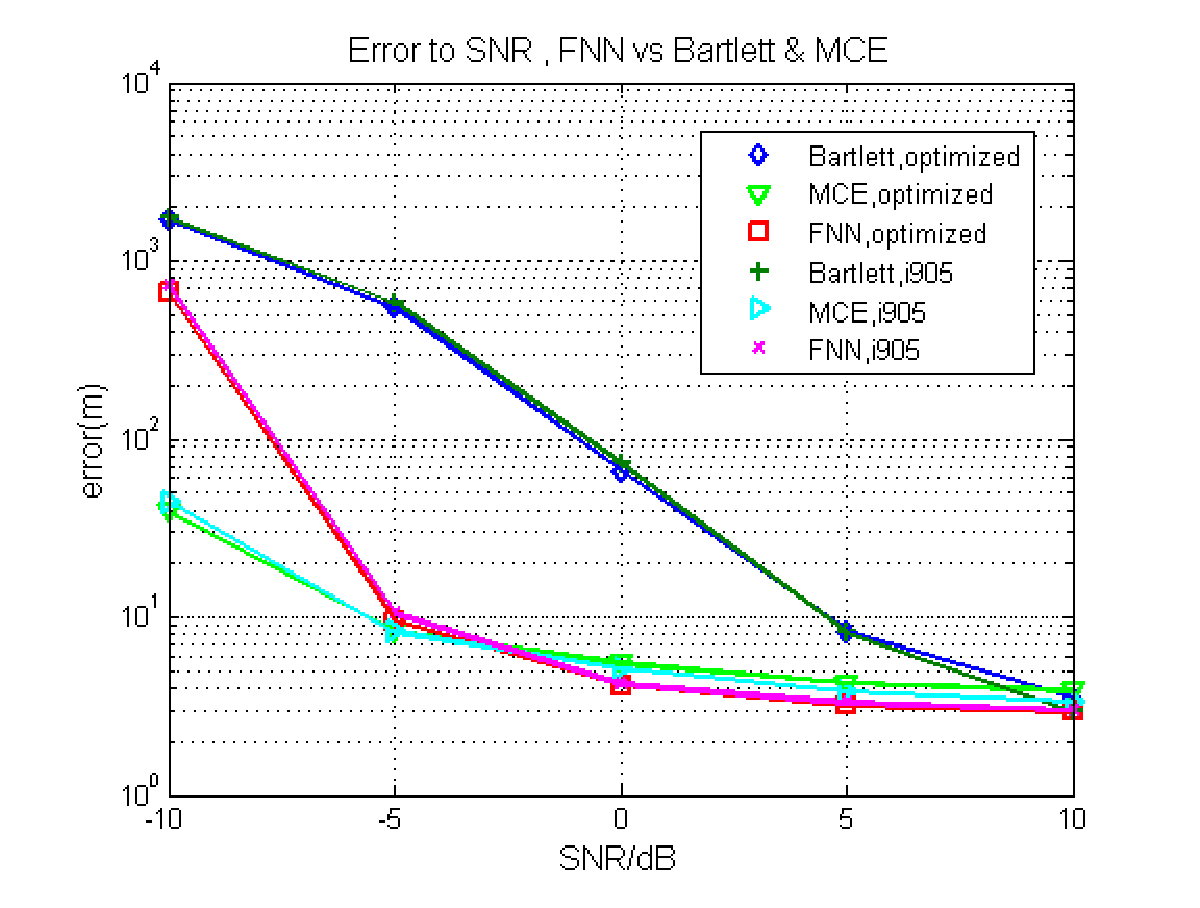
\includegraphics[width=4cm,height=3cm]{figure/Error_to_SNR_FNN_vs_Bartlett_MCE}
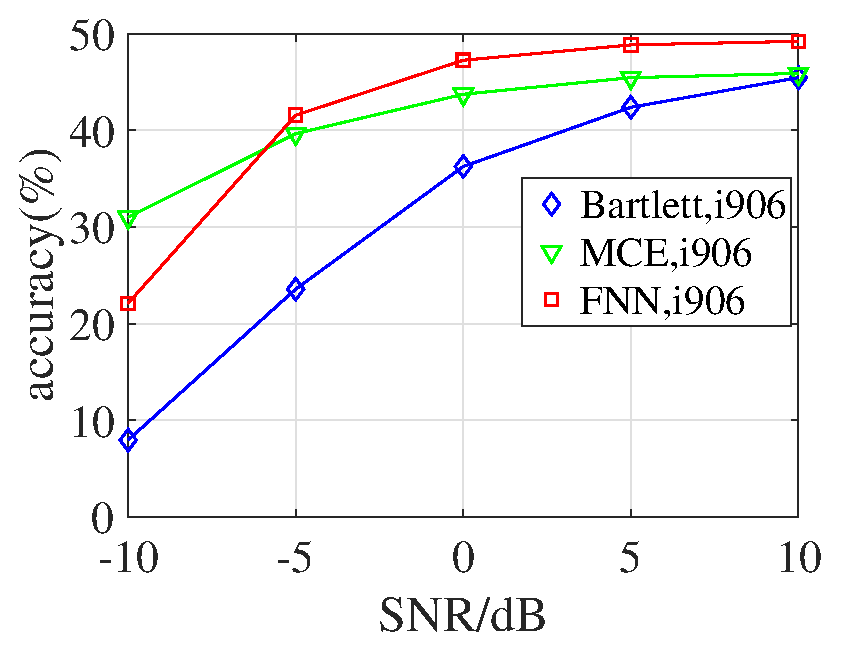
\includegraphics[width=4cm,height=3cm]{figure/Accuracy_to_SNR_FNN_vs_Bartlett_MCE_i906}
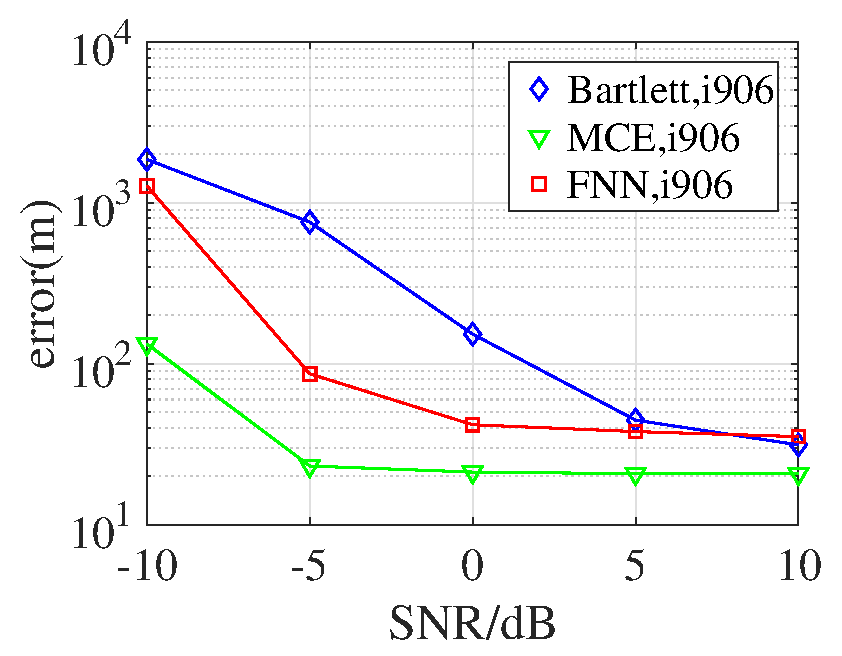
\includegraphics[width=4cm,height=3cm]{figure/Error_to_SNR_FNN_vs_Bartlett_MCE_i906}
\caption{FNN positioning performance curve on simulation data(frequency:109,232,385Hz).
 FNN is also sensitive to SSP mismatch, but still performs better than Bartlett.
}
\end{figure}
The performance curves for SCFNN, Bartlett and MCE vs SNR are plotted by 1000 times Monte Carlo simulation in Fig. 6. The snapshot here is 10.
Simulation results show that when the change in SSP is relatively slight, SCFNN positioning best, followed by MCE and Bartlett worst and when the change is relatively large (existing shape varying), the accuracy order is unchanged, but the absolute mean error of SCFNN becomes bigger than MCE.
This is maybe caused by the noisy training data.
In conclusion, SCFNN is also sensitive to SSP mismatch, but still performs better than Bartlett and the performance of SCFNN is close to the MCE methods.
\begin{figure}
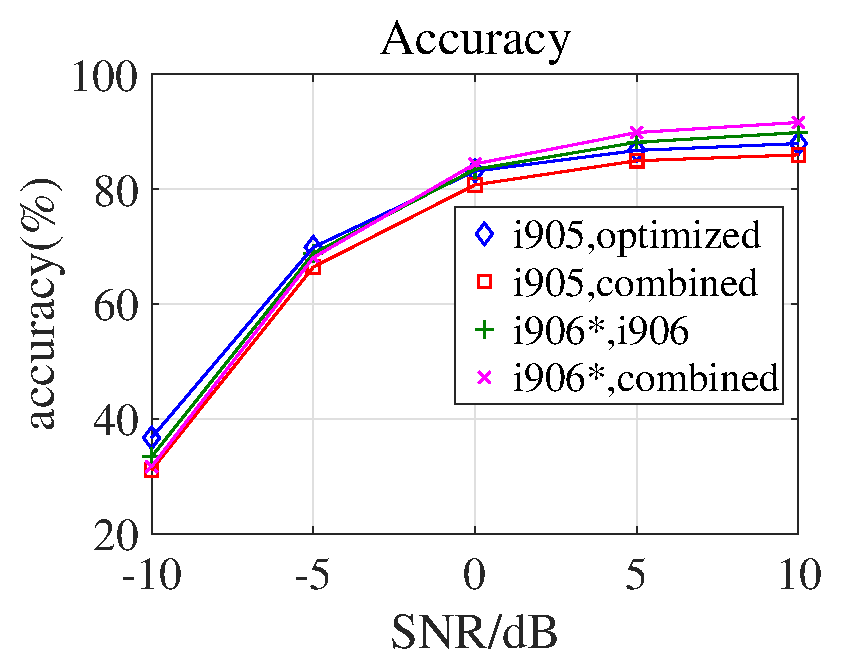
\includegraphics[width=4cm,height=3cm]{figure/Accuracy_to_SNR_Combined_vs_Single}
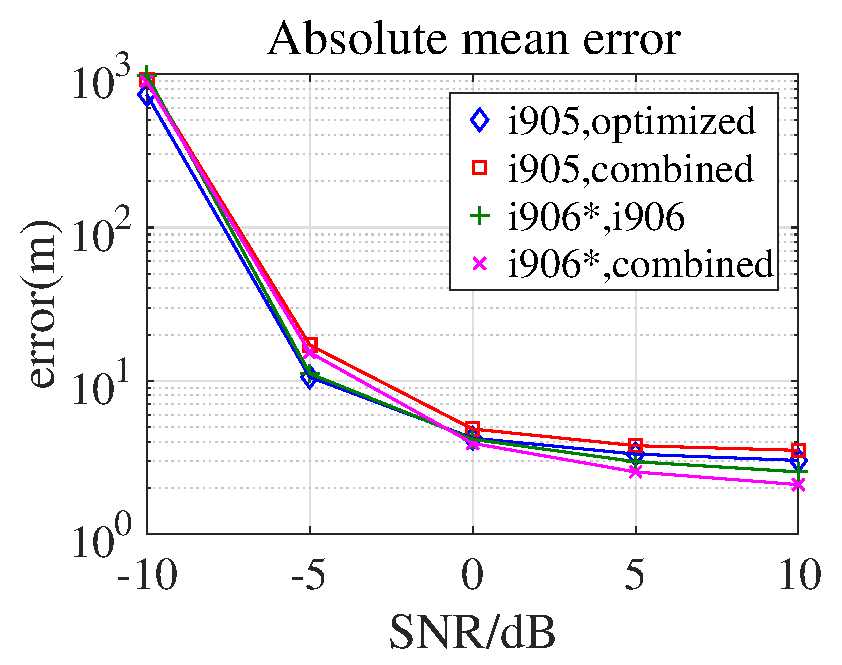
\includegraphics[width=4cm,height=3cm]{figure/Error_to_SNR_Combined_vs_Single}
\caption{FNN positioning performance curve on simulation data. FNN model robustness can be by significantly improved by data-model mixed training}
\end{figure}

\subsection{%Co-training using data collected from different ssp
Increase model robustness by data-model mixed training}
%\begin{figure}
%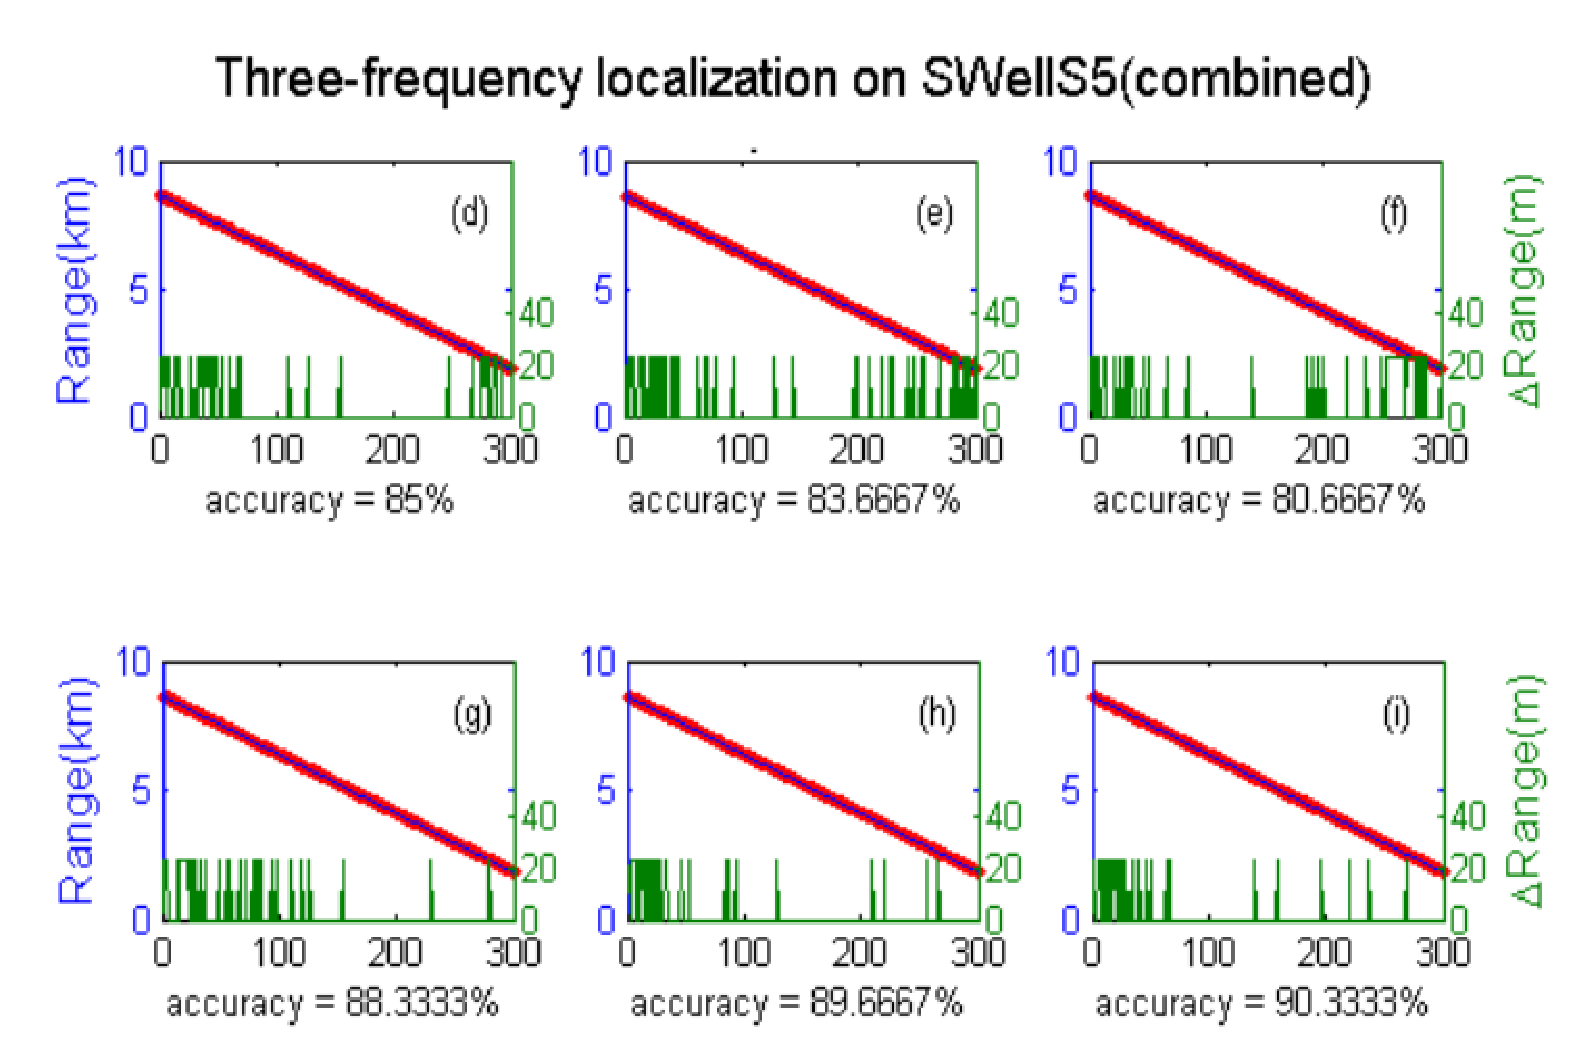
\includegraphics[width=4cm,height=3cm]{figure/combinevssingle_lef}
%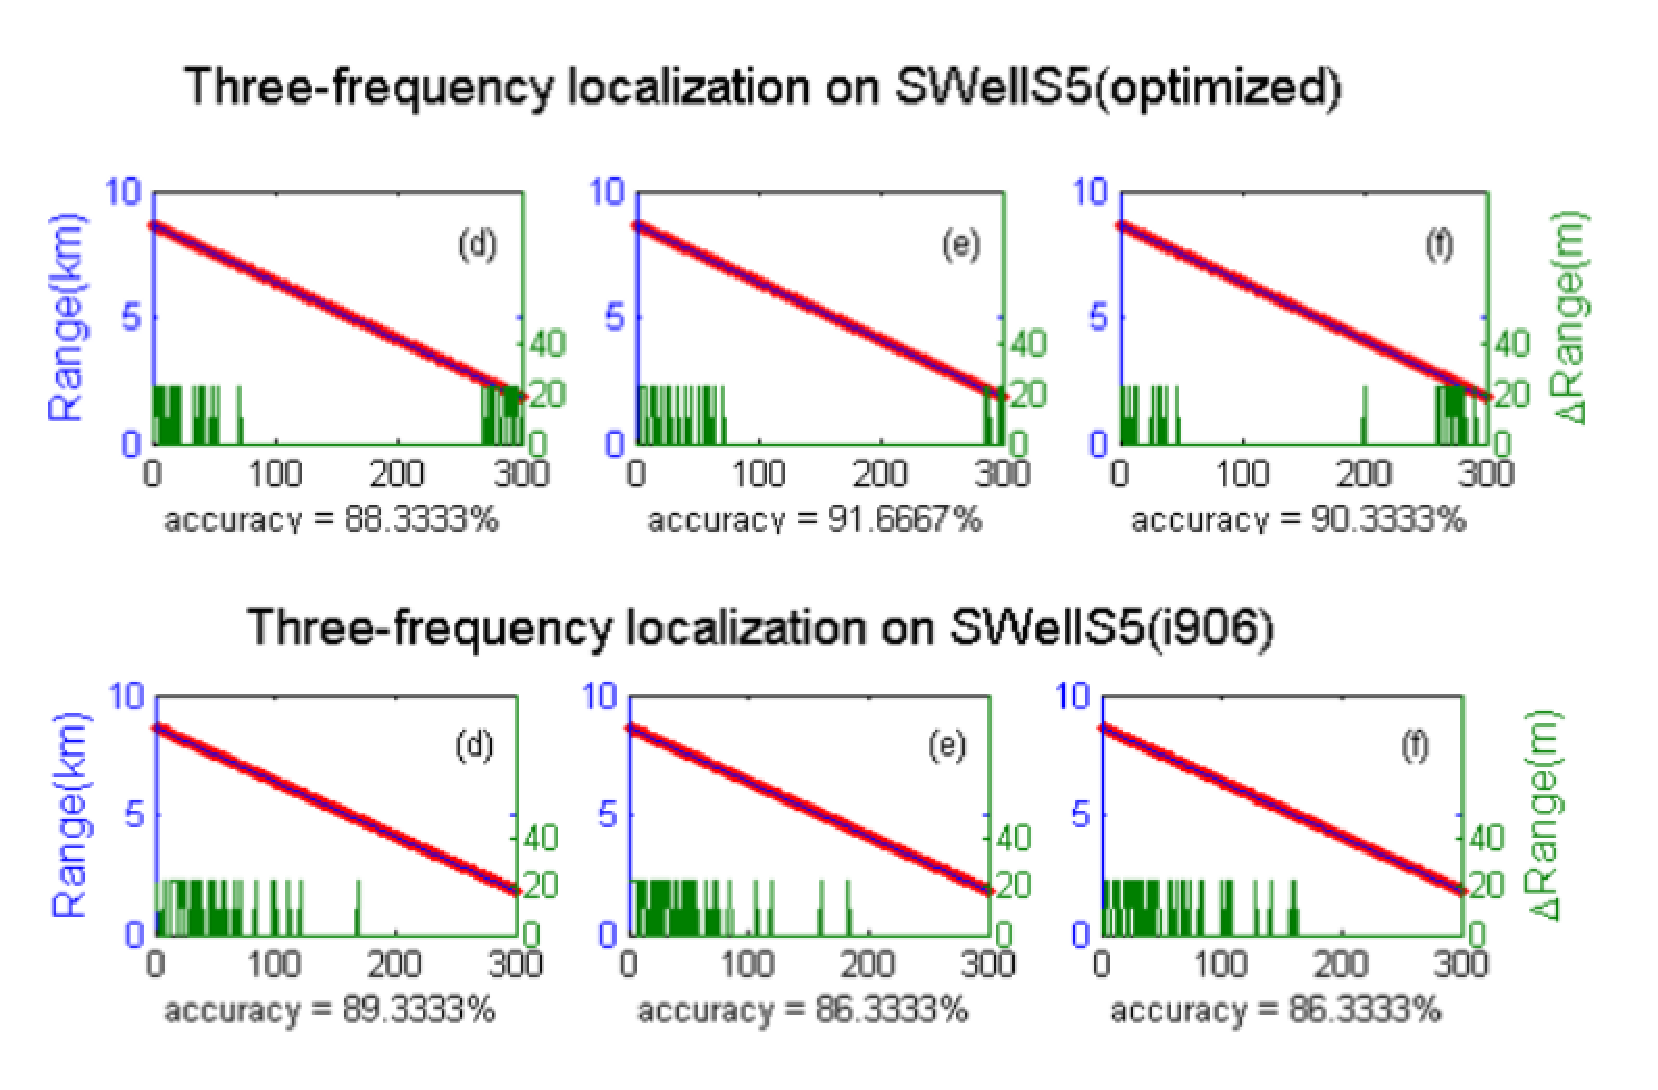
\includegraphics[width=4cm,height=3cm]{figure/combinevssingle_right}
%\caption{Comparison of mixed data training and single data training .}
%\end{figure}
As mentioned in section 3.4, the SCFNN is also sensitive to SSP mismatch. When the environment SSP has a big change in shape, the classifier trained by single data set performs poorly.
For example, the model trained by data set corresponding to ssp-optimized, performs poorly on ssp-i906{*}, and the accuracy drops about 40\%, compared with the performance on ssp-i905. In this section, by combining the data collected from ssp-i906 and ssp-optimized as training set, the robustness of the classifier increases significantly, as Fig. 7 shows, the re-trained classifier predicts accurately on ssp-i906{*}, just as well as on ssp-i905.
Although the accuracy for i905 has a little glissade compared with single data training case, the performance for i906 improved. By mixed data-model training, the SCFNN classifier works well on two entirely different SSPs. Note that, in Fig. 7, the legend `i905,combined'  means the model is trained by mixed data, and then tested on ssp-i905. The rest legends are similar.
%The simulation results show that training the model using data collected from different SSP can significantly improve the robustness of the classifier, which means FNN can learn weights over a set of changing SSP.
\section{Summary}
In this paper, we propose a method that can help solve the mismatch problem in matched-field source localization,
by using a sparsely-coded feed-forward neural network(SCFNN), combined with data-model mixed training.
The proposal is examined on SWellEx-96 experiment.
To be specific, we firstly train and test a prediction model on the experimental data,
and confirm that the SCFNN works well on source localization.
Then, the influence of SSP mismatch on the SCFNN classifier is investigated by simulations. Finally, we train the SCFNN with mixed environment model data.
It is attractive to see that the model robustness is significantly improved and the trained classifier performs well on varying SSP environments.

Comparing with dense neural networks, the sparsely-code neural network needs fewer basis functions to span the data space and
is beneficial to capture characteristic of data distributions, which will make the model be more descriptive.
% and is helpful to capture characteristic of data distributions.

The discussion on applying machine learning methods for overcoming mismatch problem in underwater source localization is preliminary and only a fine-tuned FNN is used in this paper. Machine learning has potential advantages in unstable underwater acoustics, it deserves more efforts to research deeper.

%\begin{acks}
%The work is supported by ...
%\end{acks}
